% background chapter continued

\addtocontents{toc}{\protect\setcounter{tocdepth}{1}}

\section{Crawl Ordering Problem}
The purpose of a web crawler can be viewed as traversing the web graph. The crawling order appears naturally
to be breath-first problem (download pages following the links as they appear). But since the web is so
massive and still expanding such a crawling activity is considered infinite and the crawler itself can
be said to be \textit{random walker} with no purpose. Most of the commercial or even open source crawlers
have some sort of crawling order policy built into their system. It is a must for small-scale, special
purpose crawler to order the extracted URLs because the act of acquiring content is restricted by various
factors.
\\
\\
Figure \ref{fig:crawlorder} shows how different types of crawls tradeoff page importance.
\\
\begin{figure}[h!]
  \centering
  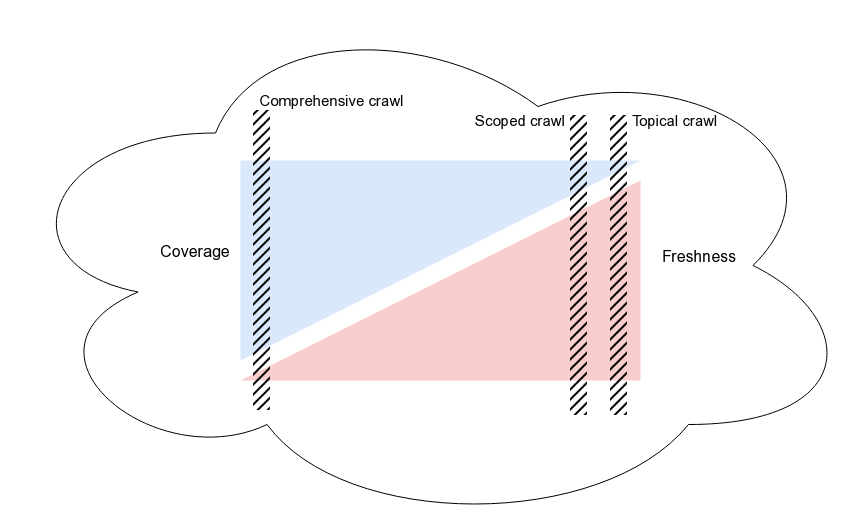
\includegraphics[width=15cm,height=12cm,keepaspectratio]{../media/crawler/crawl-ordering.png}
  \caption{Crawl ordering based on Coverage vs. Freshness}
  \label{fig:crawlorder}
\end{figure}

\begin{description}
\textbf{Coverage:} Focus is on fetching pages that crawler deems required. \leavemode \\
\\
\textbf{Freshness:} Here the focus is on revisting, redownloading already visited pages. Since web 2.0,
pages are capable of dynamically changing content and upcoming web 3.0 will have javascript rendered data.
\\
\\
The question of balancing content coverage and freshness in a crawler is solely a decision of entity behind
it.
\end{description}
\\
 

\subsection{Batch Crawling}

\subsection{Incremental Crawling}


\addtocontents{toc}{\protect\setcounter{tocdepth}{3}}

